\documentclass{ximera}
\usepackage{multicol}

\title{Continuity Activity}
\author{MATH 425: Calculus I}

\begin{document}
\begin{abstract}
     Working with the peers in your group, solve the following problems. Make sure to show and justify all your work. Make sure everyone in the group understands the solution and participates. Be prepared to report your answers to the whole class. 
\end{abstract}
\maketitle

\begin{exercise}
     Decide if each of the five given statements is true or false.  If the statement is false, provide a counterexample: sketch a graph of a function showing that the statement is false.  Then use another representation: a table, a symbolic equation, and/or words to explain why the graph you sketched disproves the statement. 
    \begin{enumerate}
        \item If $\lim_{x\rightarrow c}f(x)=f(c)$, then $f$ is continuous at $x=c$.  \\
        We think this statement is true / false\\
        Justification (explain with words, a table, an equation or graph, OR provide a counterexample, if applicable):
        \item If $f$ is not continuous at $x=c$, then $f(x)\neq \lim_{x\rightarrow c}f(x)$.\\
        We think this statement is true / false\\
        Justification (explain with words, a table, an equation or graph, OR provide a counterexample, if applicable):
        \item If $f$ is not continuous at $x=c$, then $f(c)$ is undefined.\\
        We think this statement is true / false\\
        Justification (explain with words, a table, an equation or graph, OR provide a counterexample, if applicable):
        \item If $f$ is not continuous at $x=c$, then $\lim_{x\rightarrow c}f(x)$ does not exist.\\
        We think this statement is true / false\\
        Justification (explain with words, a table, an equation or graph, OR provide a counterexample, if applicable):
        \item If $f$ is not continuous at $x=c$, then either $f(c)$ is undefined or $\lim_{x\rightarrow c}f(x)$ does not exist.\\
        We think this statement is true / false\\
        Justification (explain with words, a table, an equation or graph, OR provide a counterexample, if applicable):
        \item Which statements in part (a) through (e) match the following graphs:
        
      
        \begin{image}
        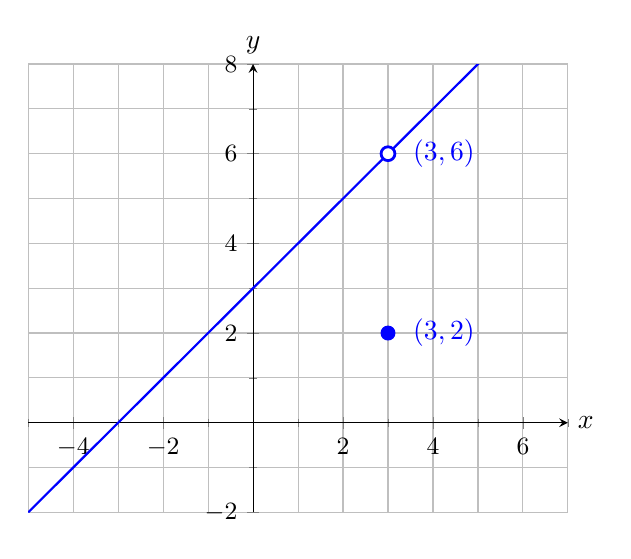
\begin{tikzpicture}
  \begin{axis}[
    axis lines=middle,
    xlabel={$x$},
    ylabel={$y$},
    xmin=-5, xmax=7,
    ymin=-2, ymax=8,
    grid=both,
    minor tick num=1,
    enlargelimits=false,
    ticklabel style={font=\small},
    every axis x label/.style={at={(current axis.right of origin)}, anchor=west},
    every axis y label/.style={at={(current axis.above origin)}, anchor=south},
  ]

    % y = x + 3 for all x (we’ll mark the hole at x=3 explicitly)
    \addplot[
      domain=-5:7,
      samples=200,
      thick,
      blue
    ] {x + 3};

   % White-filled dot
\addplot[
  only marks,
  mark=*,
  mark size=2.5pt,
  draw=none,
  fill=white
] coordinates {(3,6)};

% Blue ring on top
\addplot[
  only marks,
  mark=o,
  mark size=2.5pt,
  line width=1pt,
  draw=blue
] coordinates {(3,6)};
   

    % Filled dot at (3,2) for the defined value y=2 when x=3
    \addplot[
      only marks,
      mark=*,
      mark size=2.5pt,
      blue
    ] coordinates {(3,2)};

    % Optional: labels near the special points
    \node[anchor=west, blue] at (axis cs:3,6) {$\;\;(3,6)$};
    \node[anchor=west, blue]  at (axis cs:3,2) {$\;\;(3,2)$};

  \end{axis}
  
\end{tikzpicture}

\end{image}
    Graph A\\
    
\begin{image}
        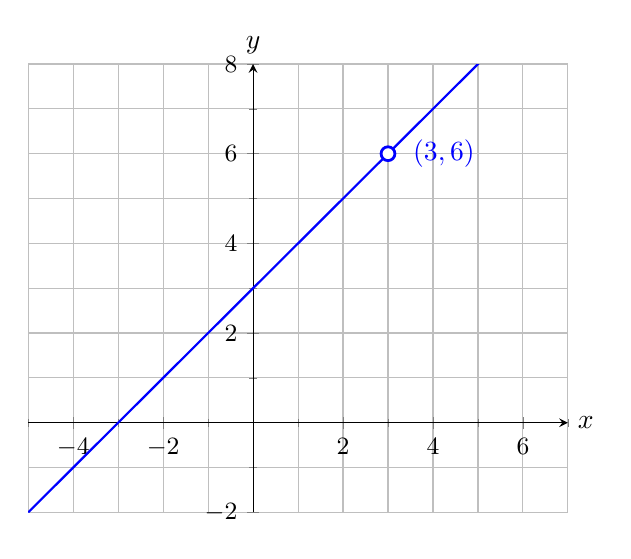
\begin{tikzpicture}
  \begin{axis}[
    axis lines=middle,
    xlabel={$x$},
    ylabel={$y$},
    xmin=-5, xmax=7,
    ymin=-2, ymax=8,
    grid=both,
    minor tick num=1,
    enlargelimits=false,
    ticklabel style={font=\small},
    every axis x label/.style={at={(current axis.right of origin)}, anchor=west},
    every axis y label/.style={at={(current axis.above origin)}, anchor=south},
  ]

    % y = x + 3 for all x (we’ll mark the hole at x=3 explicitly)
    \addplot[
      domain=-5:7,
      samples=200,
      thick,
      blue
    ] {x + 3};

    % White-filled dot
\addplot[
  only marks,
  mark=*,
  mark size=2.5pt,
  draw=none,
  fill=white
] coordinates {(3,6)};

% Blue ring on top
\addplot[
  only marks,
  mark=o,
  mark size=2.5pt,
  line width=1pt,
  draw=blue
] coordinates {(3,6)};
   

    % Optional: labels near the special points
    \node[anchor=west, blue] at (axis cs:3,6) {$\;\;(3,6)$};
    %\node[anchor=west, blue]  at (axis cs:3,2) {$\;\;(3,2)$};

  \end{axis}
 
\end{tikzpicture}

        \end{image}
        Graph B\\

        We think graph A matches with ...\\
        We think graph B matches with ... \\
        (Question modified from Straumanis et al., \textit{Calculus I: A Guided Inquiry}, 2014.)
    \end{enumerate}
\end{exercise}

\begin{exercise}
    Give an example of a single function $f(x)$ such that satisfies the following four characteristics:\\
    \begin{enumerate} 
        \item $f(x)$ is continuous everywhere except at $x=-2, 3$ and $4$
        \item $f(3)=5$
        \item $\lim_{x\rightarrow 2^-}f(x)=1$
        \item $\lim_{x\rightarrow 4}f(x)=6$
    \end{enumerate}

    (Hint: A symbolic equation is not the only way to represent a function.  A sketch of a graph may be an easier representation to use here.)\\
    (Questions modified from Boelkins, et al., \textit{Active Calculus}, 1st ed.)
\end{exercise}

\end{document}